\documentclass[UTF8]{article} 
\usepackage{graphicx}
\usepackage{subfigure}
\usepackage{amsmath}
\usepackage{makecell}
\usepackage[utf8]{inputenc}
\usepackage[space]{ctex} %中文包
\usepackage{listings} %放代码
\usepackage{xcolor} %代码着色宏包
\usepackage{CJK} %显示中文宏包
\usepackage{float}


\definecolor{mygreen}{rgb}{0,0.6,0}
\definecolor{mygray}{rgb}{0.5,0.5,0.5}
\definecolor{mymauve}{rgb}{0.58,0,0.82}
\lstset{
	backgroundcolor=\color{white}, 
	%\tiny < \scriptsize < \footnotesize < \small < \normalsize
	basicstyle = \scriptsize,
	breakatwhitespace = false,        
	breaklines = true,                 
	captionpos = b,                    
	commentstyle = \color{mygreen}\bfseries,
	extendedchars = false,             
	frame =shadowbox, 
	framerule=0.5pt,
	keepspaces=true,
	keywordstyle=\color{blue}\bfseries, % keyword style
	language = Verilog,                     % the language of code
	otherkeywords={string}, 
	numbers=left, 
	numbersep=5pt,
	numberstyle=\tiny\color{mygray},
	rulecolor=\color{black},         
	showspaces=false,  
	showstringspaces=false, 
	showtabs=false,    
	stepnumber=1,         
	stringstyle=\color{mymauve},        % string literal style
	tabsize=4,          
	title=\lstname                      
}


\title{中国科学技术大学计算机学院\\《数字电路实验》报告}
\author{}

\date{}

\begin{document}
	\maketitle
	\begin{figure}[H]
		\centering
		
\includegraphics[width=2.5in]{xiaohui.jpg}\vspace{0.5cm}\\
		\large{
			实验题目:信号处理及有限状态机\\
			学生姓名:王章瀚\\
			学生学号:PB18111697\\
			完成日期:\today\\
		}\vspace{2cm}
		
		\large{计算机实验教学中心制\\2019年09月\\}
		\thispagestyle{empty}
		\clearpage  % 清除当页页码
	\end{figure}


	\section{实验目的}
	进一步熟悉 FPGA 开发的整体流程\par
	掌握几种常见的信号处理技巧\par
	掌握有限状态机的设计方法\par
	能够使用有限状态机设计功能电路\par
	
	\section{实验环境}
	PC 一台\par
	Windows 或 Linux 操作系统\par
	VivadoFPGA 实验平台(Nexys4 DDR)\par
	Logisim\par
	vlab.ustc.edu.cn\par
	
	\section{实验过程}
	\subsection{信号去抖动}
	在用 FPGA 开发板的按键或开关作为输入时,由于其机械特性,在电平转换的瞬间会产生一些抖动,这些抖动在用户看来非常短暂,但在 100MHz 的时钟信号下会持续许多个周期。\par
	而消除抖动的关键在于区分有效的按键输入和按键按下或抬起瞬间的机械抖动。以人的反应速度来看,按键按下再抬起,最快也在毫秒以上量级,而抖动一般都在微秒甚至纳秒量级,因此我们可以通过信号电平持续时间的长短来判定是否为一次有效按键。\par
	讲义给出的代码通过计数器来计时,达到累加阈值后停止计数。\par
	以下是我的仿真结果:\par
	\begin{figure}[H]
		\centering
		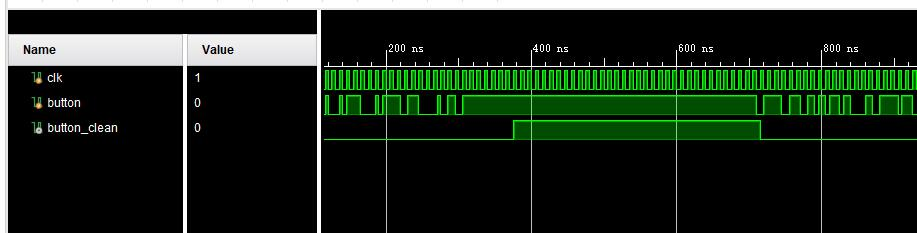
\includegraphics[width=1\linewidth]{s1_1.jpg}
		\label{s1_1}
	\end{figure}\par
	通过去抖动电路,我们能够将信号电平转换过程中的“毛刺”消除掉,使得输入信号变得更加干净、可靠。\par

	\subsection{取信号边沿技巧}
	很多电子设备都是用按键或开关等外设控制电路状态的跳转,但除了时钟和异步复位信号外,其它信号都不应放在边沿敏感列表内,因此可以用类似下面的代码实现:\par
	\begin{lstlisting}[language=Verilog]
	always@(posedge clk)
		if(控制信号==1)
			//状态跳转
		else
			//状态保持
	\end{lstlisting}\par
	但是这要求该信号为持续时间为一个时钟周期的脉冲信号,否则电路状态会一直跳转。 \par
	因此可以用下述方法,通过该按键信号生成一个时钟周期宽度的脉冲信号。\par
	\begin{figure}[H]
		\centering
		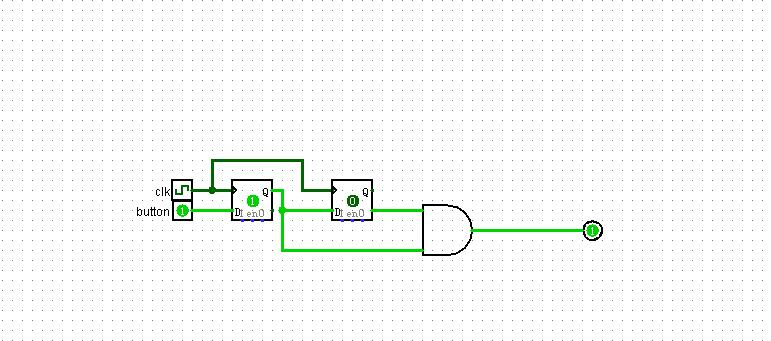
\includegraphics[width=1\linewidth]{s2_1.jpg}
		\label{s2_1}
	\end{figure}\par
	这样能够产生下面这样的波形:\par
	\begin{figure}[H]
		\centering
		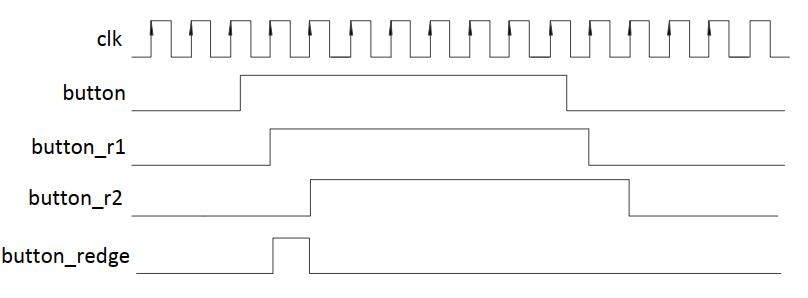
\includegraphics[width=1\linewidth]{s2_2.jpg}
		\label{s2_2}
	\end{figure}\par

	\subsection{有限状态机介绍}
	一般来说,数字电路由组合逻辑和时序逻辑构成。 典型的数字电路都可以归结为以下两种基本结构:\par
	\begin{figure}[H]
		\centering
		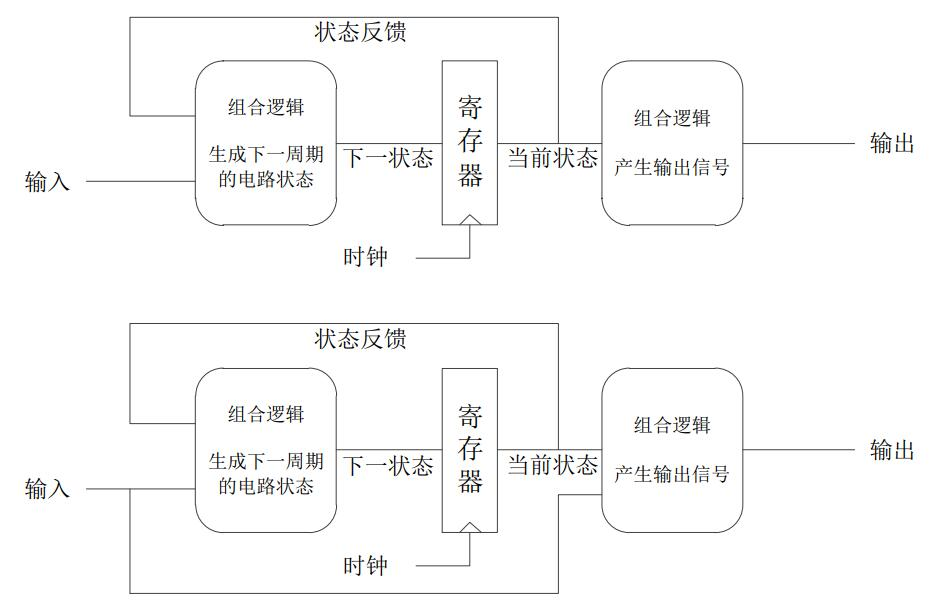
\includegraphics[width=0.7\linewidth]{s3_1.jpg}
		\label{s3_1}
	\end{figure}\par
	其状态数量是有限的,因此这种电路结构称为有限状态机。\par
	有限状态机分为摩尔型(Moore)和米利型(Mealy)。\par
	Moore 型时序更好,但响应要慢一拍, Mealy 型响应最快, 但时序上要差一些。一般来说,如果对电路相应速度要求不是非常苛刻的话,推荐使用 Moore 型有限状态机。\par
	例如,红绿灯的电路,其输入信号为计时信号(timer\_pulse),该信号为持续一个时钟周期的脉冲信号,输出信号为绿灯 (green\_light)。 电路包含 3 种状态(PASS、 TRANS、 STOP,分别用2’b00,2’b01,2’b10 表示), 复位状态为“PASS”。 \par
	最终设计得到如下电路图:\par
	\begin{figure}[H]
		\centering
		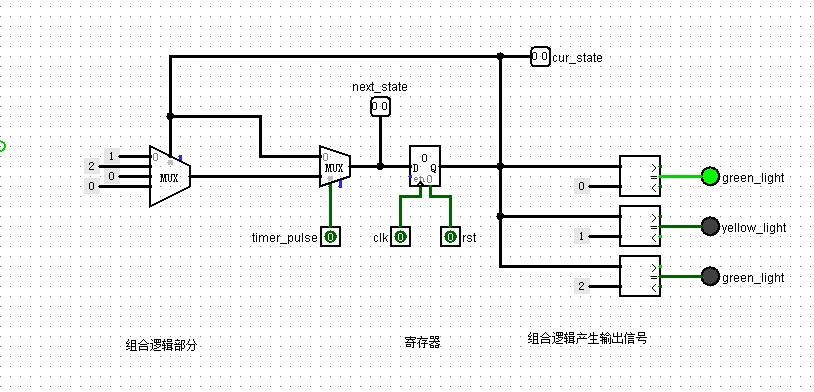
\includegraphics[width=0.7\linewidth]{s3_2.jpg}
		\label{s3_2}
	\end{figure}\par

	\subsection{有限状态机 Verilog 实现}
	将上述三部分:1.纯组合逻辑部分,2.时序逻辑部分,3.组合逻辑输出部分,用Verilog实现。\par
	可以将整个代码划分为三大块。分别在不同的always之类的语句中实现。这叫三段式写法。当然还有更多不同的写法,如两段式和一段式,但代码层次结构和可读性要比三段式写法差一些。
	
	\subsection{有限状态机的另一形式}
	有时候代码并不会严格按照有限状态机的三段式格式来写,但也确实是个摩尔型有限状态机(或米利型)。\par
	比如下面这个代码:\par
	\begin{lstlisting}[language=Verilog]
	module test(
		input clk,rst,
		output led);
		reg [1:0] cnt;
		
	always@(posedge clk or posedge rst)
	begin
		if(rst)
			cnt <= 2'b0;
		else
			cnt <= cnt + 1'b1;
	end
	assign led = (cnt==2'b11) ? 1'b1 : 1'b0;
	endmodule
	\end{lstlisting}
	该电路包含了 4 个状态(0,1, 2, 3) , 电路在这 4 个状态之间循环跳转, 其中加法器用于生成次态(cnt+1) ,寄存器将次态信号传递给现态(cnt) ,最后的比较器通过现态信号生成输出信号(led) 。 \par
	确实是个摩尔型有限状态机。\par
	

	\section{实验练习}
	\subsection{题目1}
	代码如下:\par
	\begin{lstlisting}[language=Verilog]
	module e1(
		input clk,rst,
		output led);
	
	parameter STATE0 = 2'b00;
	parameter STATE1 = 2'b01;
	parameter STATE2 = 2'b10;
	parameter STATE3 = 2'b11;
	reg [1:0] cur_state = 0;
	reg [1:0] next_state = 0;
	
	// set the next_state.
	always @(*)
	begin
		case(cur_state)
			STATE0: next_state <= STATE1;
			STATE1: next_state <= STATE2;
			STATE2: next_state <= STATE3;
			STATE3: next_state <= STATE0;
			default: next_state <= STATE0;
		endcase
	end
	
	// the sequential part
	always@(posedge clk or posedge rst)
	begin
		if(rst)
			cur_state <= STATE0;
		else
			cur_state <= next_state;
	end
	
	// output part
	assign led = (cur_state==STATE3) ? 1'b1 : 1'b0;
	
	endmodule
	\end{lstlisting}
	可以得到仿真结果如下:\par
	\begin{figure}[H]
		\centering
		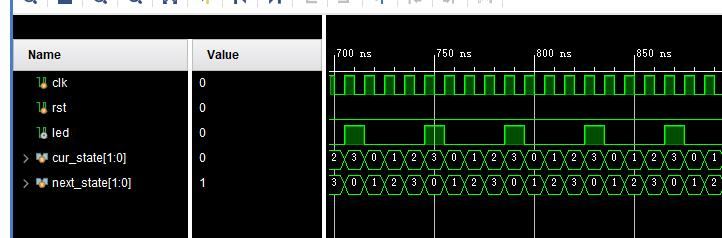
\includegraphics[width=1\linewidth]{e1_1.jpg}
		\label{e1_1}
	\end{figure}\par
	
	\subsection{题目2}
	上升下降沿都要自加,因此使用两个寄存器,而对应不同边沿用Mux选取不同寄存器。如下图:\par
	\begin{figure}[H]
		\centering
		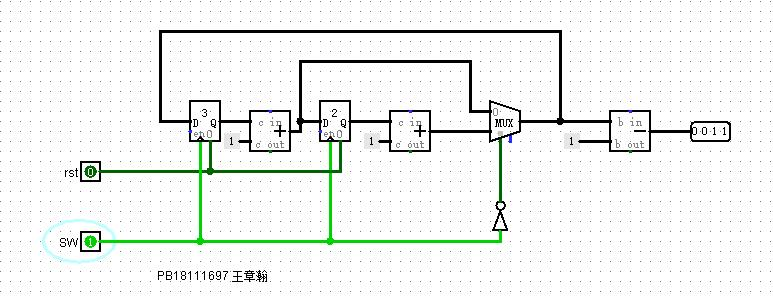
\includegraphics[width=1\linewidth]{e2.jpg}
		\label{e2}
	\end{figure}\par

	\subsection{题目3}
	按照题意,应该设计的是按键产生边沿触发来计数。\par
	下面是一个没有加消抖的代码,事实上这样一个简单的程序不加消抖,在实际烧入后的操作中,似乎并没有影响。以下是不加消抖的代码(后面还有加了消抖的):\par
	\begin{lstlisting}[language=Verilog]
	module e3(
		input clk, BTNU, BTND, rst,
		output [7:0] seg,
		output reg [7:0] AN
		);
	
	integer cnt_target_1000HZ = 100000;
	integer cnt_1000HZ = 0;
	
	reg [3:0] data = 0;
	dist_mem_gen_0 dist_mem_gen_0(data, seg);
	
	reg [8:0] cnt = 0;
	reg BTNU1, BTNU2;
	reg BTND1, BTND2;
	wire BTNU_redge, BTND_redge;
	
	// 构造良好边沿
	always @(posedge clk) BTNU1 <= BTNU;
	always @(posedge clk) BTNU2 <= BTNU1;
	always @(posedge clk) BTND1 <= BTND;
	always @(posedge clk) BTND2 <= BTND1;
	assign BTNU_redge = ~BTNU2 & BTNU1;
	assign BTND_redge = ~BTND2 & BTND1;
	
	always @(negedge clk or posedge rst)
	begin
		if(rst)
			cnt <= 8'h1F;
		else
		begin
			if(BTNU_redge)
				cnt = cnt + 1;
			if(BTND_redge)
				cnt = cnt - 1;
		end
	end
	
	// 时分复用
	always @(posedge clk)
	begin
		cnt_1000HZ = cnt_1000HZ + 1;
		if(cnt_1000HZ == cnt_target_1000HZ)
		begin
			cnt_1000HZ <= 0;
			case(AN)
				8'b1111_1101 : begin AN <= 8'b1111_1110; data <= cnt[3:0]; end
				default : begin AN <= 8'b1111_1101; data <= cnt[7:4]; end
			endcase
		end
	end
	
	endmodule
	\end{lstlisting}
	加了消抖的代码:\par
	\begin{lstlisting}[language=Verilog]
	module e3(
		input clk, BTNU, BTND, rst,
		output [7:0] seg,
		output reg [7:0] AN
		);
	
	integer cnt_target_1000HZ = 100000;
	integer cnt_1000HZ = 0;
	
	reg [3:0] data = 0;
	dist_mem_gen_0 dist_mem_gen_0(data, seg);
	
	reg [8:0] cnt = 0;
	reg BTNU0, BTNU1, BTNU2;
	reg BTND0, BTND1, BTND2;
	wire BTNU_redge, BTND_redge;
	integer BTNU_counter = 0, BTND_counter = 0;
	
	// 消抖
	always @(posedge clk)
	begin
		if(BTNU)
		begin
			if(BTNU_counter >= 100000)
			begin
				BTNU_counter <= 100000;        
				BTNU0 <= 1;
			end
			else
				BTNU_counter <= BTNU_counter + 1;
		end
		else
		begin
			BTNU_counter <= 0;
			BTNU0 <= 0;
		end
	end
	
	
	always @(posedge clk)
	begin
		if(BTND)
		begin
			if(BTND_counter >= 100000)
			begin
				BTND_counter <= 100000;        
				BTND0 <= 1;
			end
			else
				BTND_counter <= BTND_counter + 1;
		end
		else
		begin
			BTND_counter <= 0;
			BTND0 <= 0;
		end
	end
	
	// 构造良好边沿
	always @(posedge clk) BTNU1 <= BTNU0;
	always @(posedge clk) BTNU2 <= BTNU1;
	always @(posedge clk) BTND1 <= BTND;
	always @(posedge clk) BTND2 <= BTND1;
	assign BTNU_redge = ~BTNU2 & BTNU1;
	assign BTND_redge = ~BTND2 & BTND1;
	
	always @(negedge clk or posedge rst)
	begin
		if(rst)
			cnt <= 8'h1F;
		else
		begin
			if(BTNU_redge)
				cnt = cnt + 1;
			else if(BTND_redge)
				cnt = cnt - 1;
		end
	end
	
	// 时分复用
	always @(posedge clk)
	begin
		cnt_1000HZ = cnt_1000HZ + 1;
		if(cnt_1000HZ == cnt_target_1000HZ)
		begin
			cnt_1000HZ <= 0;
			case(AN)
				8'b1111_1101 : begin AN <= 8'b1111_1110; data <= cnt[3:0]; end
				default : begin AN <= 8'b1111_1101; data <= cnt[7:4]; end
			endcase
		end
	end
	
	endmodule
	\end{lstlisting}
	
	按下上下两个button可以实现向上向下计数。如下图:\par
	\begin{figure}[H]
		\begin{minipage}[H]{0.48\linewidth}
			\centering
			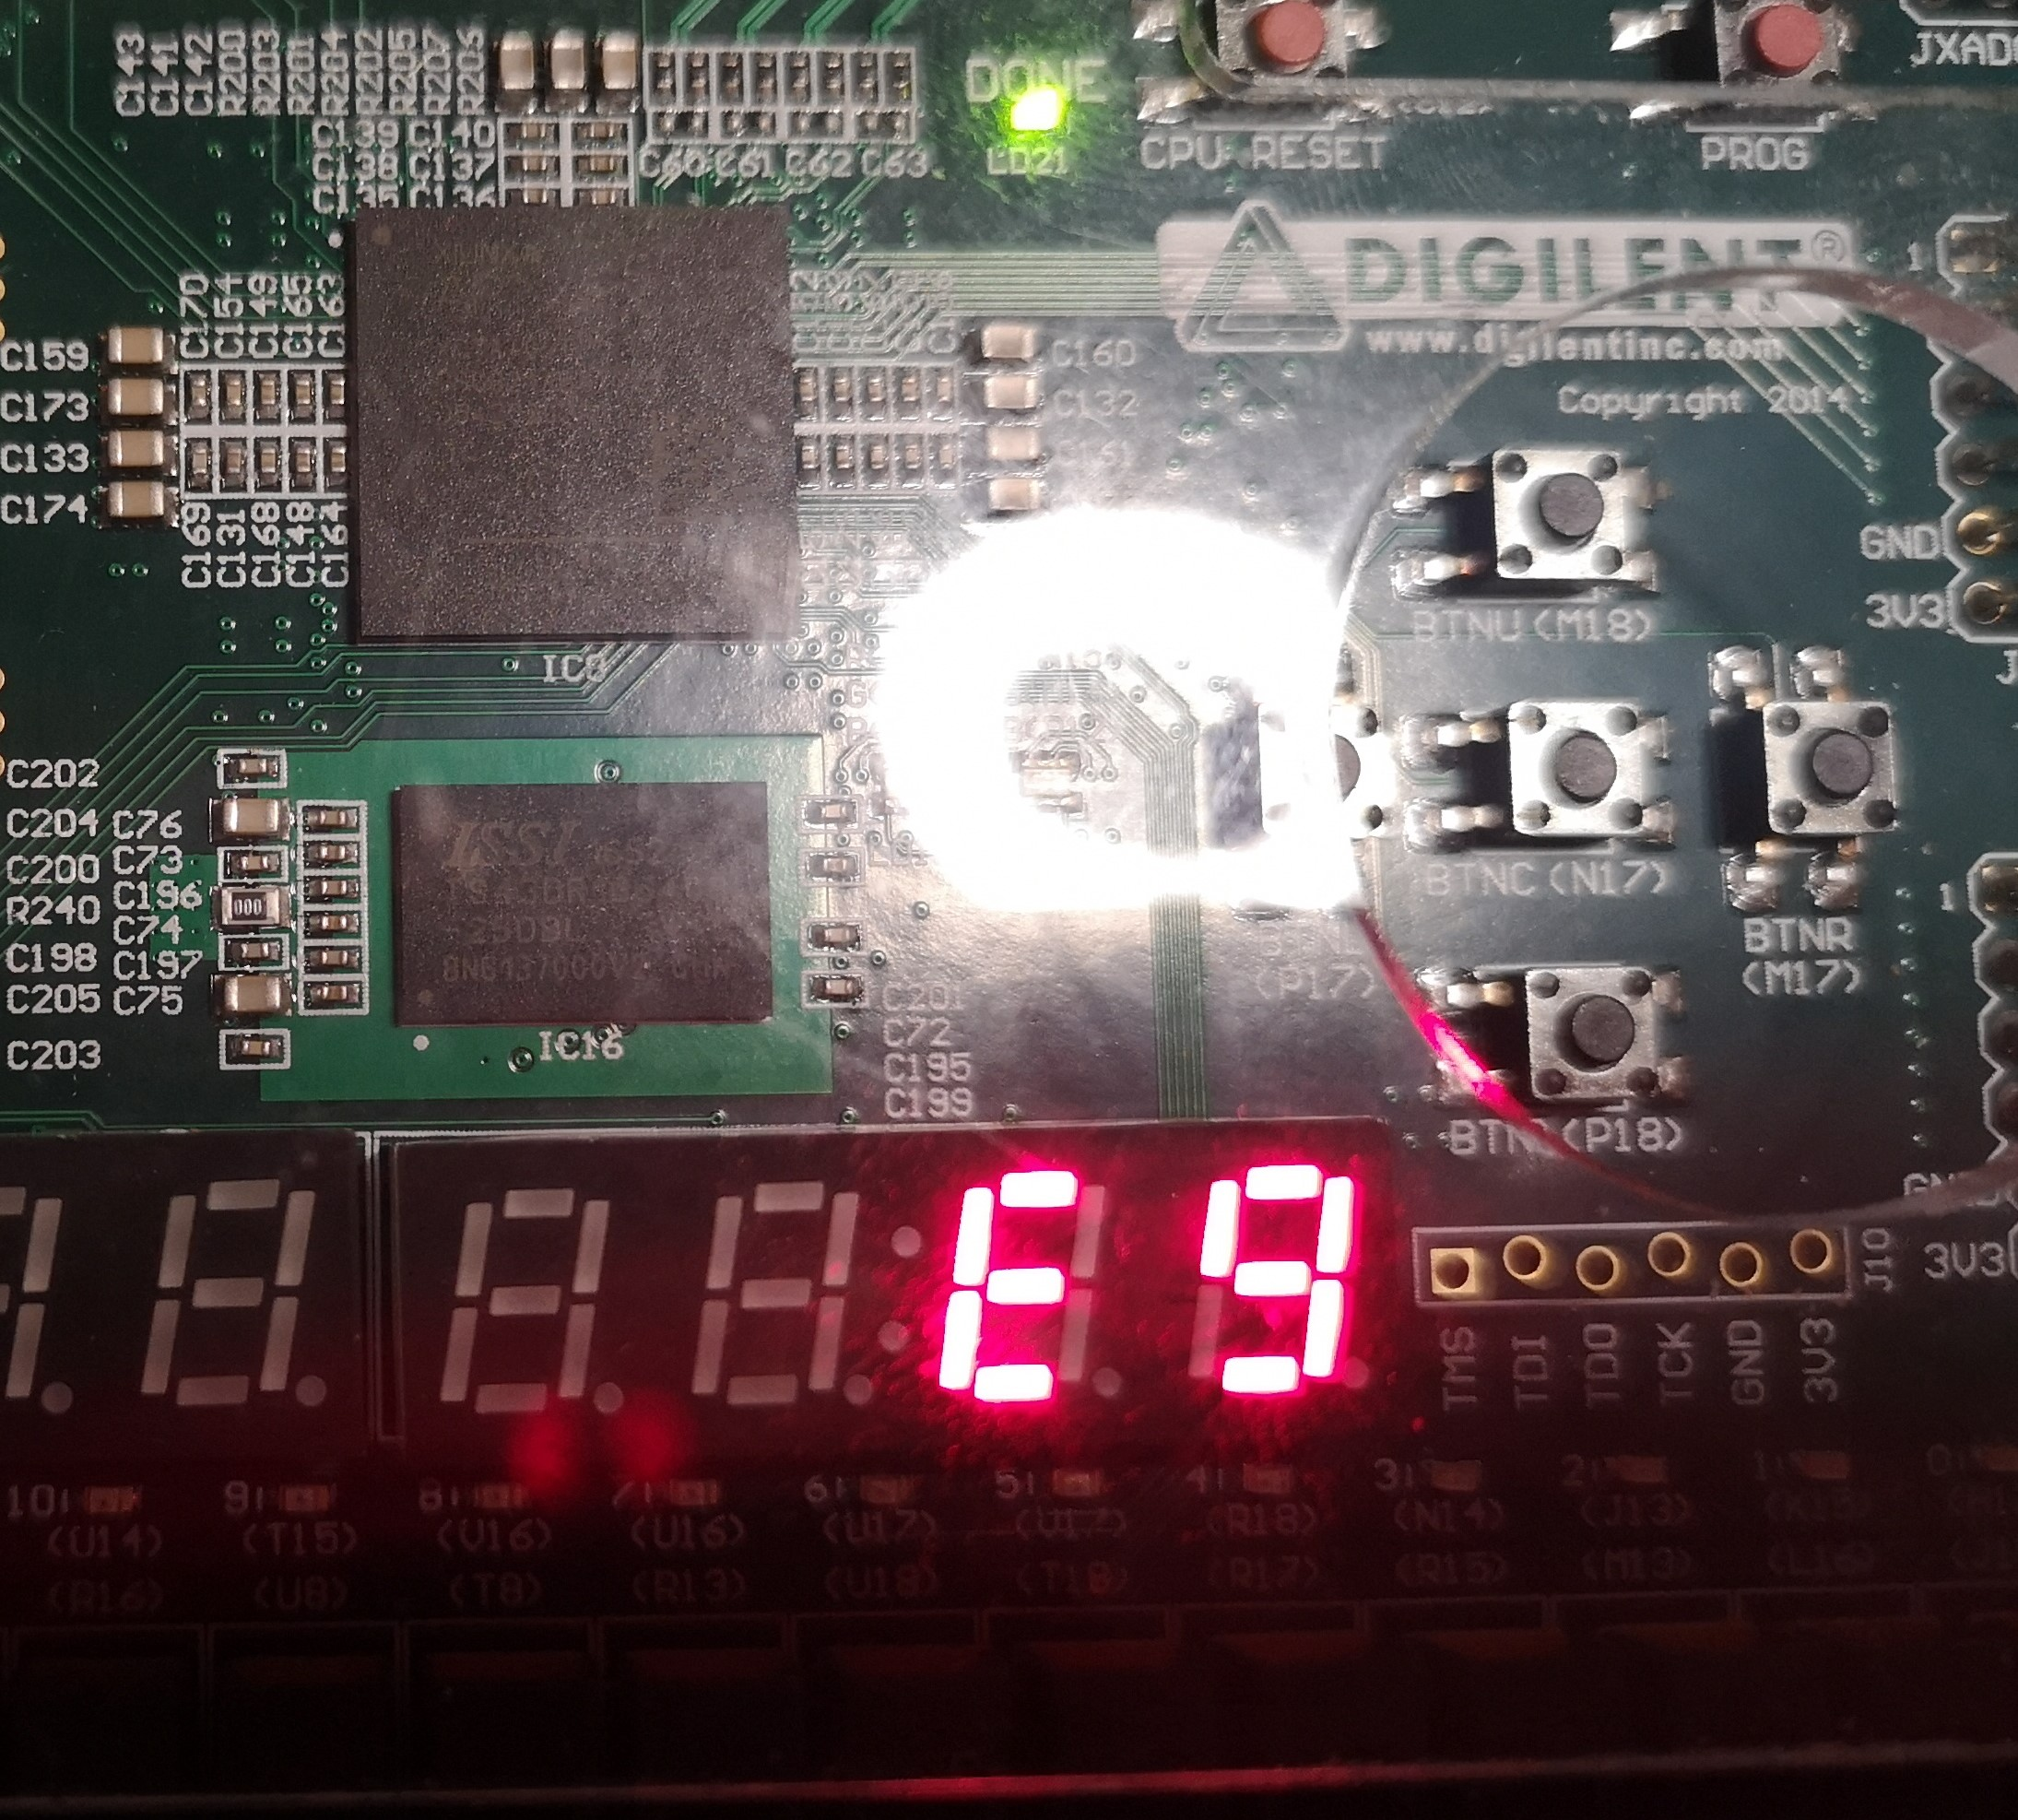
\includegraphics[scale=0.1]{e3_1.jpg}
			\label{e3_1}
		\end{minipage}
		\qquad
		\begin{minipage}[H]{0.48\linewidth}
			\centering
			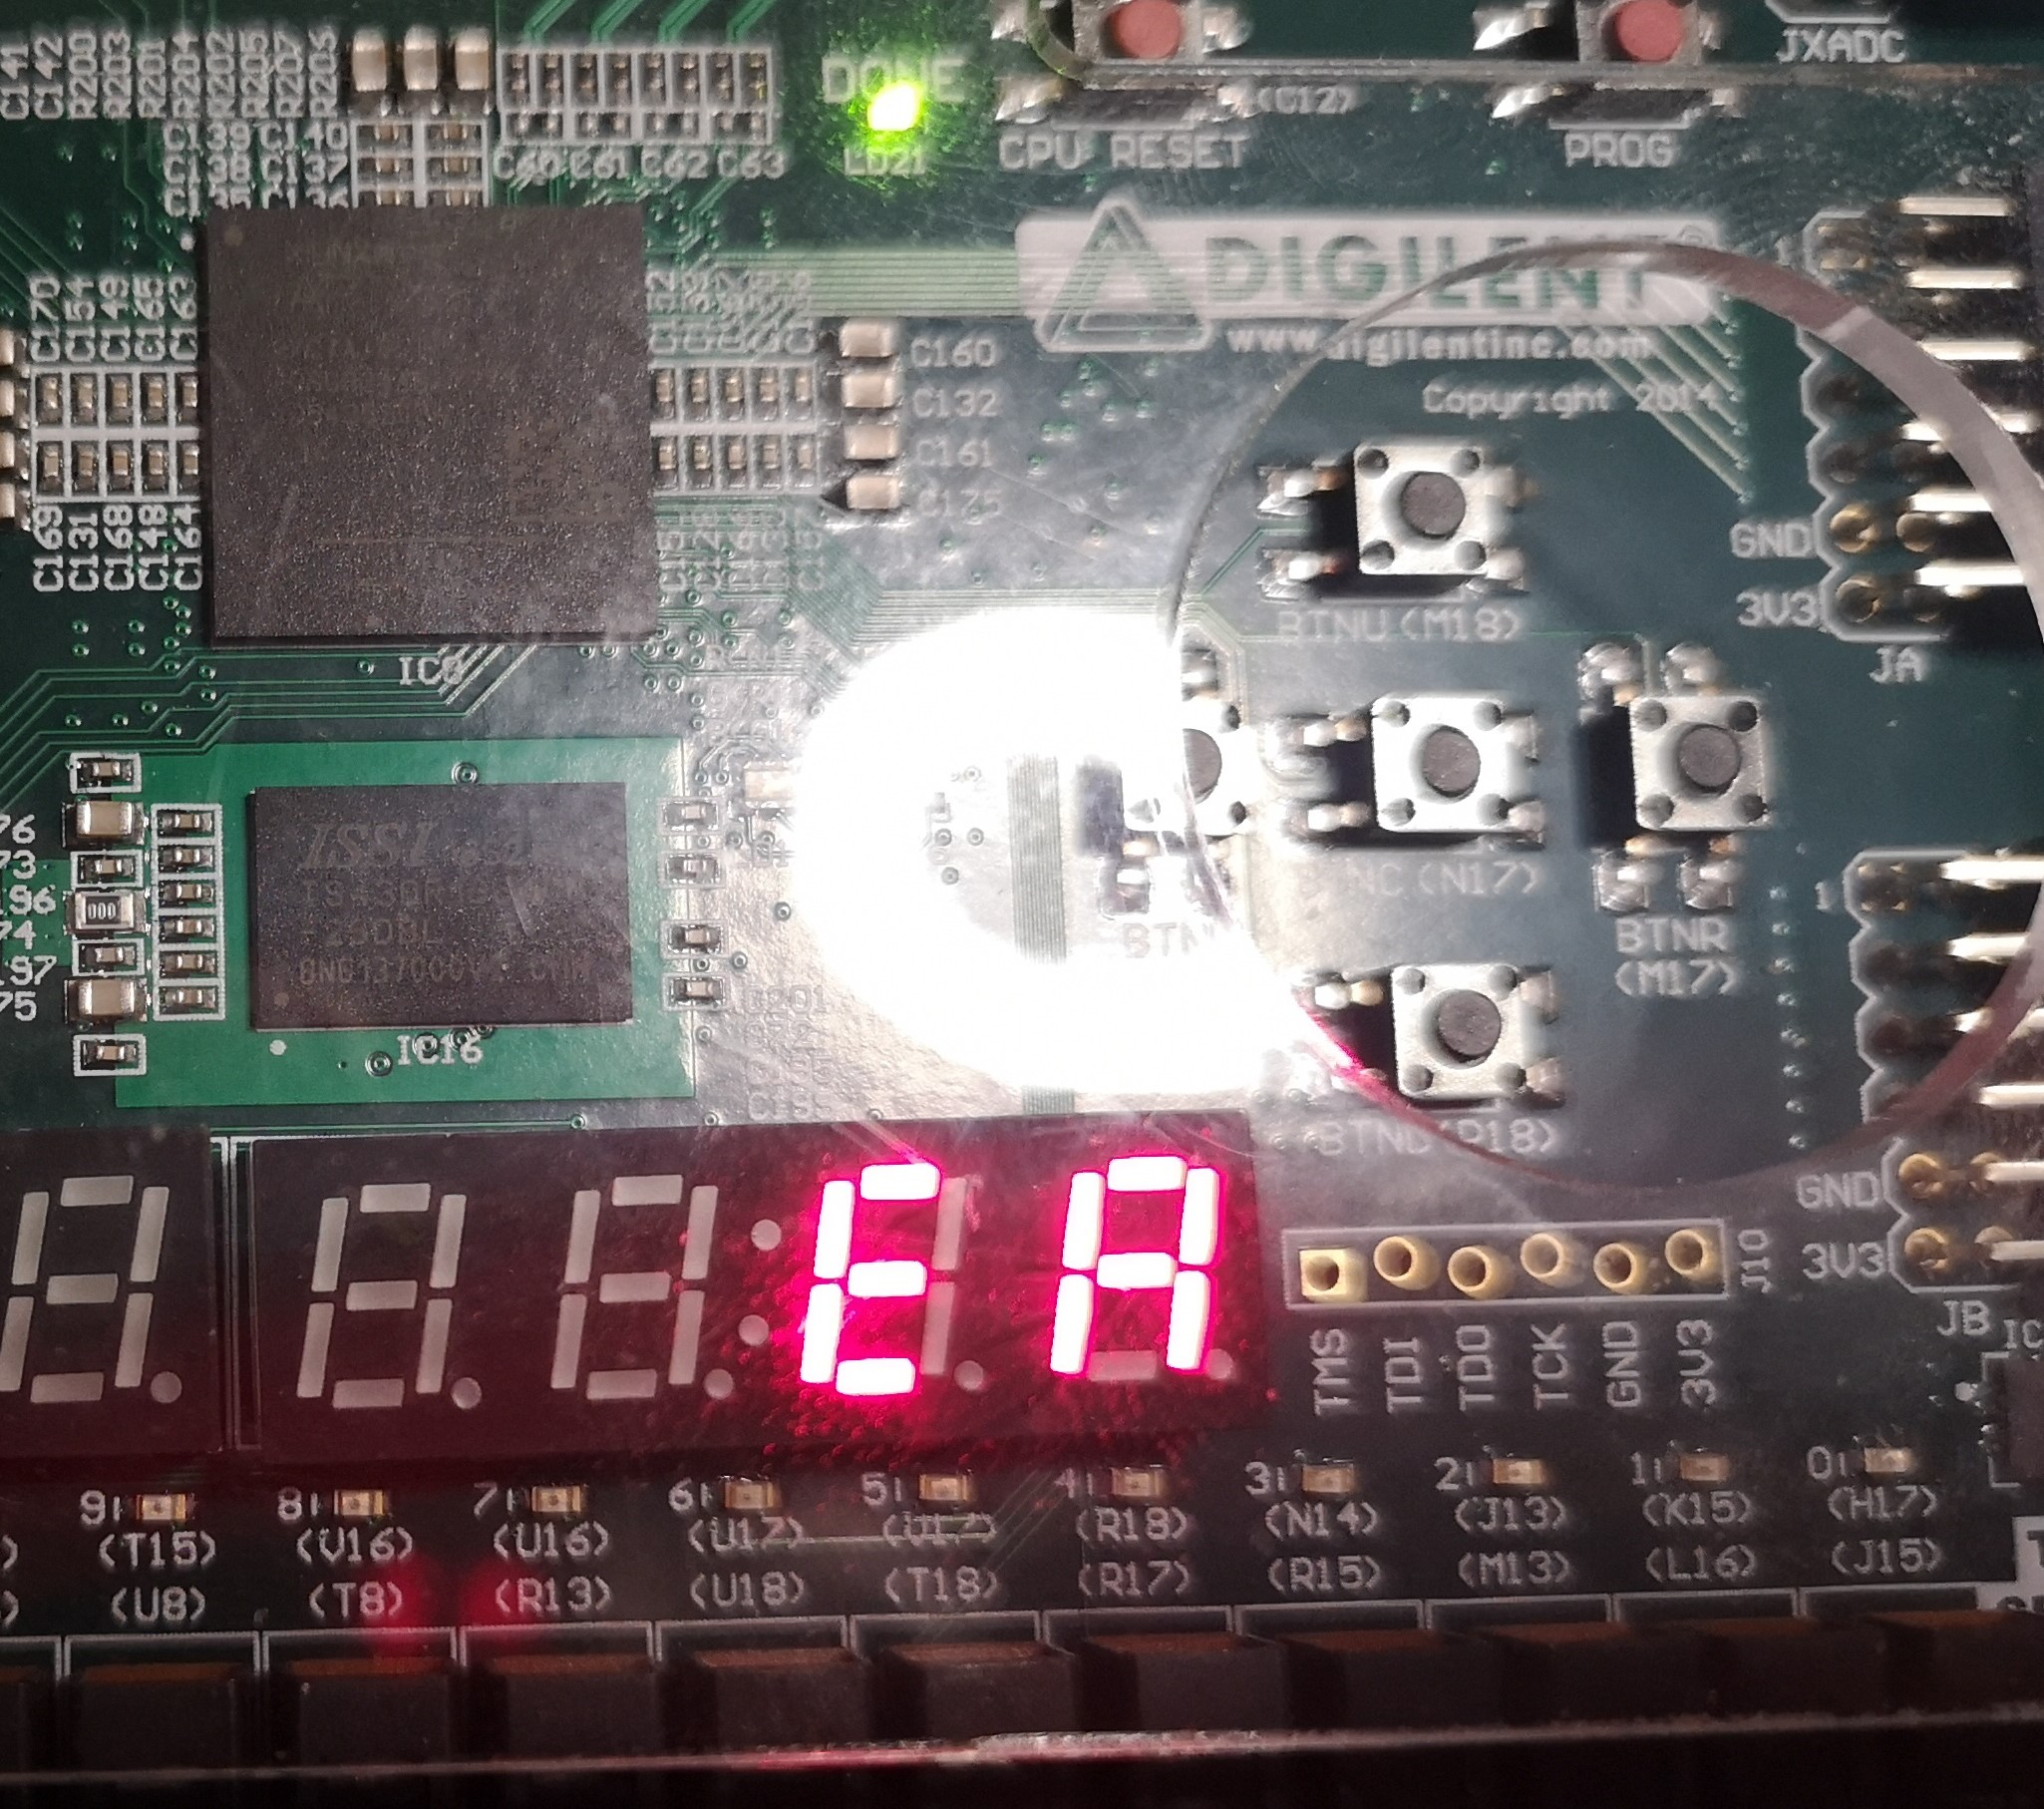
\includegraphics[scale=0.1]{e3_2.jpg}
			\label{e3_2}
		\end{minipage}
	\end{figure}

	\subsection{题目4}
	在本题中,我使用数码管7显示状态编号,数码管5显示检测到的序列数,数码管[3:0]显示最近的4个数;此外,输入的开关是SW[0],按BTNC以输入开关状态,并设置有复位键BTND。\par
	刚开始做这个题的时候,出现开关的抖动问题。后来添加了消抖程序就好了。\par
	代码如下:\par
	\begin{lstlisting}[language=Verilog]
	module e4(
		input clk, BTNC, rst, SW,
		output [7:0] seg,
		output reg [7:0] AN
		);
	
	//defination of NuxieTube's parameters.
	integer cnt_target_1000HZ, cnt_target_10HZ;
	integer cnt_1000HZ, cnt_10HZ;
	reg [3:0] last4;
	reg [3:0] data;
	
	//translate the data into seg form.
	dist_mem_gen_0 dist_mem_gen_0(data, seg);
	
	//defination of state parameters.
	reg [1:0] cur_state, next_state;
	reg [3:0] seq_counter;
	parameter SEQ_0 = 3'b000;
	parameter SEQ_1 = 3'b001;
	parameter SEQ_11 = 3'b010;
	parameter SEQ_110 = 3'b011;
	
	//debounceing and get the edge.of BTNC
	reg BTNC1, BTNC2, BTNC_0;
	integer BTNC_counter;
	wire BTNC_redge;
	always @(posedge clk)
	begin
		if(BTNC)
		begin
			if(BTNC_counter >= 100000)
			begin
				BTNC_counter <= 100000;        
				BTNC_0 <= 1;
			end
			else
				BTNC_counter <= BTNC_counter + 1;
		end
		else
		begin
			BTNC_counter <= 0;
			BTNC_0 <= 0;
		end
	end
	always @(posedge clk) BTNC1 <= BTNC_0;
	always @(posedge clk) BTNC2 <= BTNC1;
	assign BTNC_redge = BTNC1 & ~BTNC2;
	
	//some initialization
	initial
	begin
		cnt_10HZ <= 0;
		cnt_target_10HZ <= 10000000;
		cnt_10HZ <= 0;
		cnt_target_1000HZ <= 100000;
		AN <= 8'b1111_1110;
		data <= 0;
		last4 <= 16'hxxxx;
		cur_state <= SEQ_0;
		next_state <= SEQ_0;
		seq_counter <= 0;
		BTNC_counter <= 0;
	end
	
	//the sequential part
	always @(negedge clk or posedge rst)
	begin
		if(rst)
		begin
			next_state <= SEQ_0;
			seq_counter <= 4'h0;
			last4 <= 4'h0;
		end
		else if(BTNC_redge)
		begin
			//check SW, and change the state accodingly.
			if(SW) 
			begin
				case(cur_state)
					SEQ_1: next_state <= SEQ_11;
					SEQ_11: next_state <= SEQ_11;
					default: next_state <= SEQ_1;
				endcase
				last4 <= {last4[2:0], 1'b1};
			end
			else 
			begin
				case(cur_state)
					SEQ_11: next_state <= SEQ_110;
					SEQ_110: 
					begin
						next_state <= SEQ_0;
						//if 1100 is found, seq_counter++
						seq_counter <= seq_counter + 1;
					end
					default: next_state <= SEQ_0;
				endcase
				last4 <= {last4[2:0], 1'b0};
			end
		end
		else
			next_state <= cur_state;
	end
	
	//upgrade the states.
	always@(posedge clk or posedge rst)
	begin
		if(rst)
			cur_state <= SEQ_0;
		else
			cur_state <= next_state;
	end
	
	//choosing different NuxieTube.
	always @(posedge clk)
	begin
		cnt_1000HZ = cnt_1000HZ + 1;
		if(cnt_1000HZ == cnt_target_1000HZ)
		begin
			cnt_1000HZ = 0;
			case(AN)
				8'b1101_1111 : begin AN <= 8'b0111_1111; data <= {2'b00, cur_state}; end
				8'b1111_0111 : begin AN <= 8'b1101_1111; data <= seq_counter; end
				8'b1111_1011 : begin AN <= 8'b1111_0111; data <= last4[3]; end
				8'b1111_1101 : begin AN <= 8'b1111_1011; data <= last4[2]; end
				8'b1111_1110 : begin AN <= 8'b1111_1101; data <= last4[1]; end
				8'b0111_1111 : begin AN <= 8'b1111_1110; data <= last4[0]; end
				default : begin AN <= 8'b1111_1110; data <= last4[3:0]; end
			endcase
		end
	end
	
	endmodule
	\end{lstlisting}
	
	效果如下图:\par
	\begin{figure}[H]
		\begin{minipage}[H]{0.48\linewidth}
			\centering
			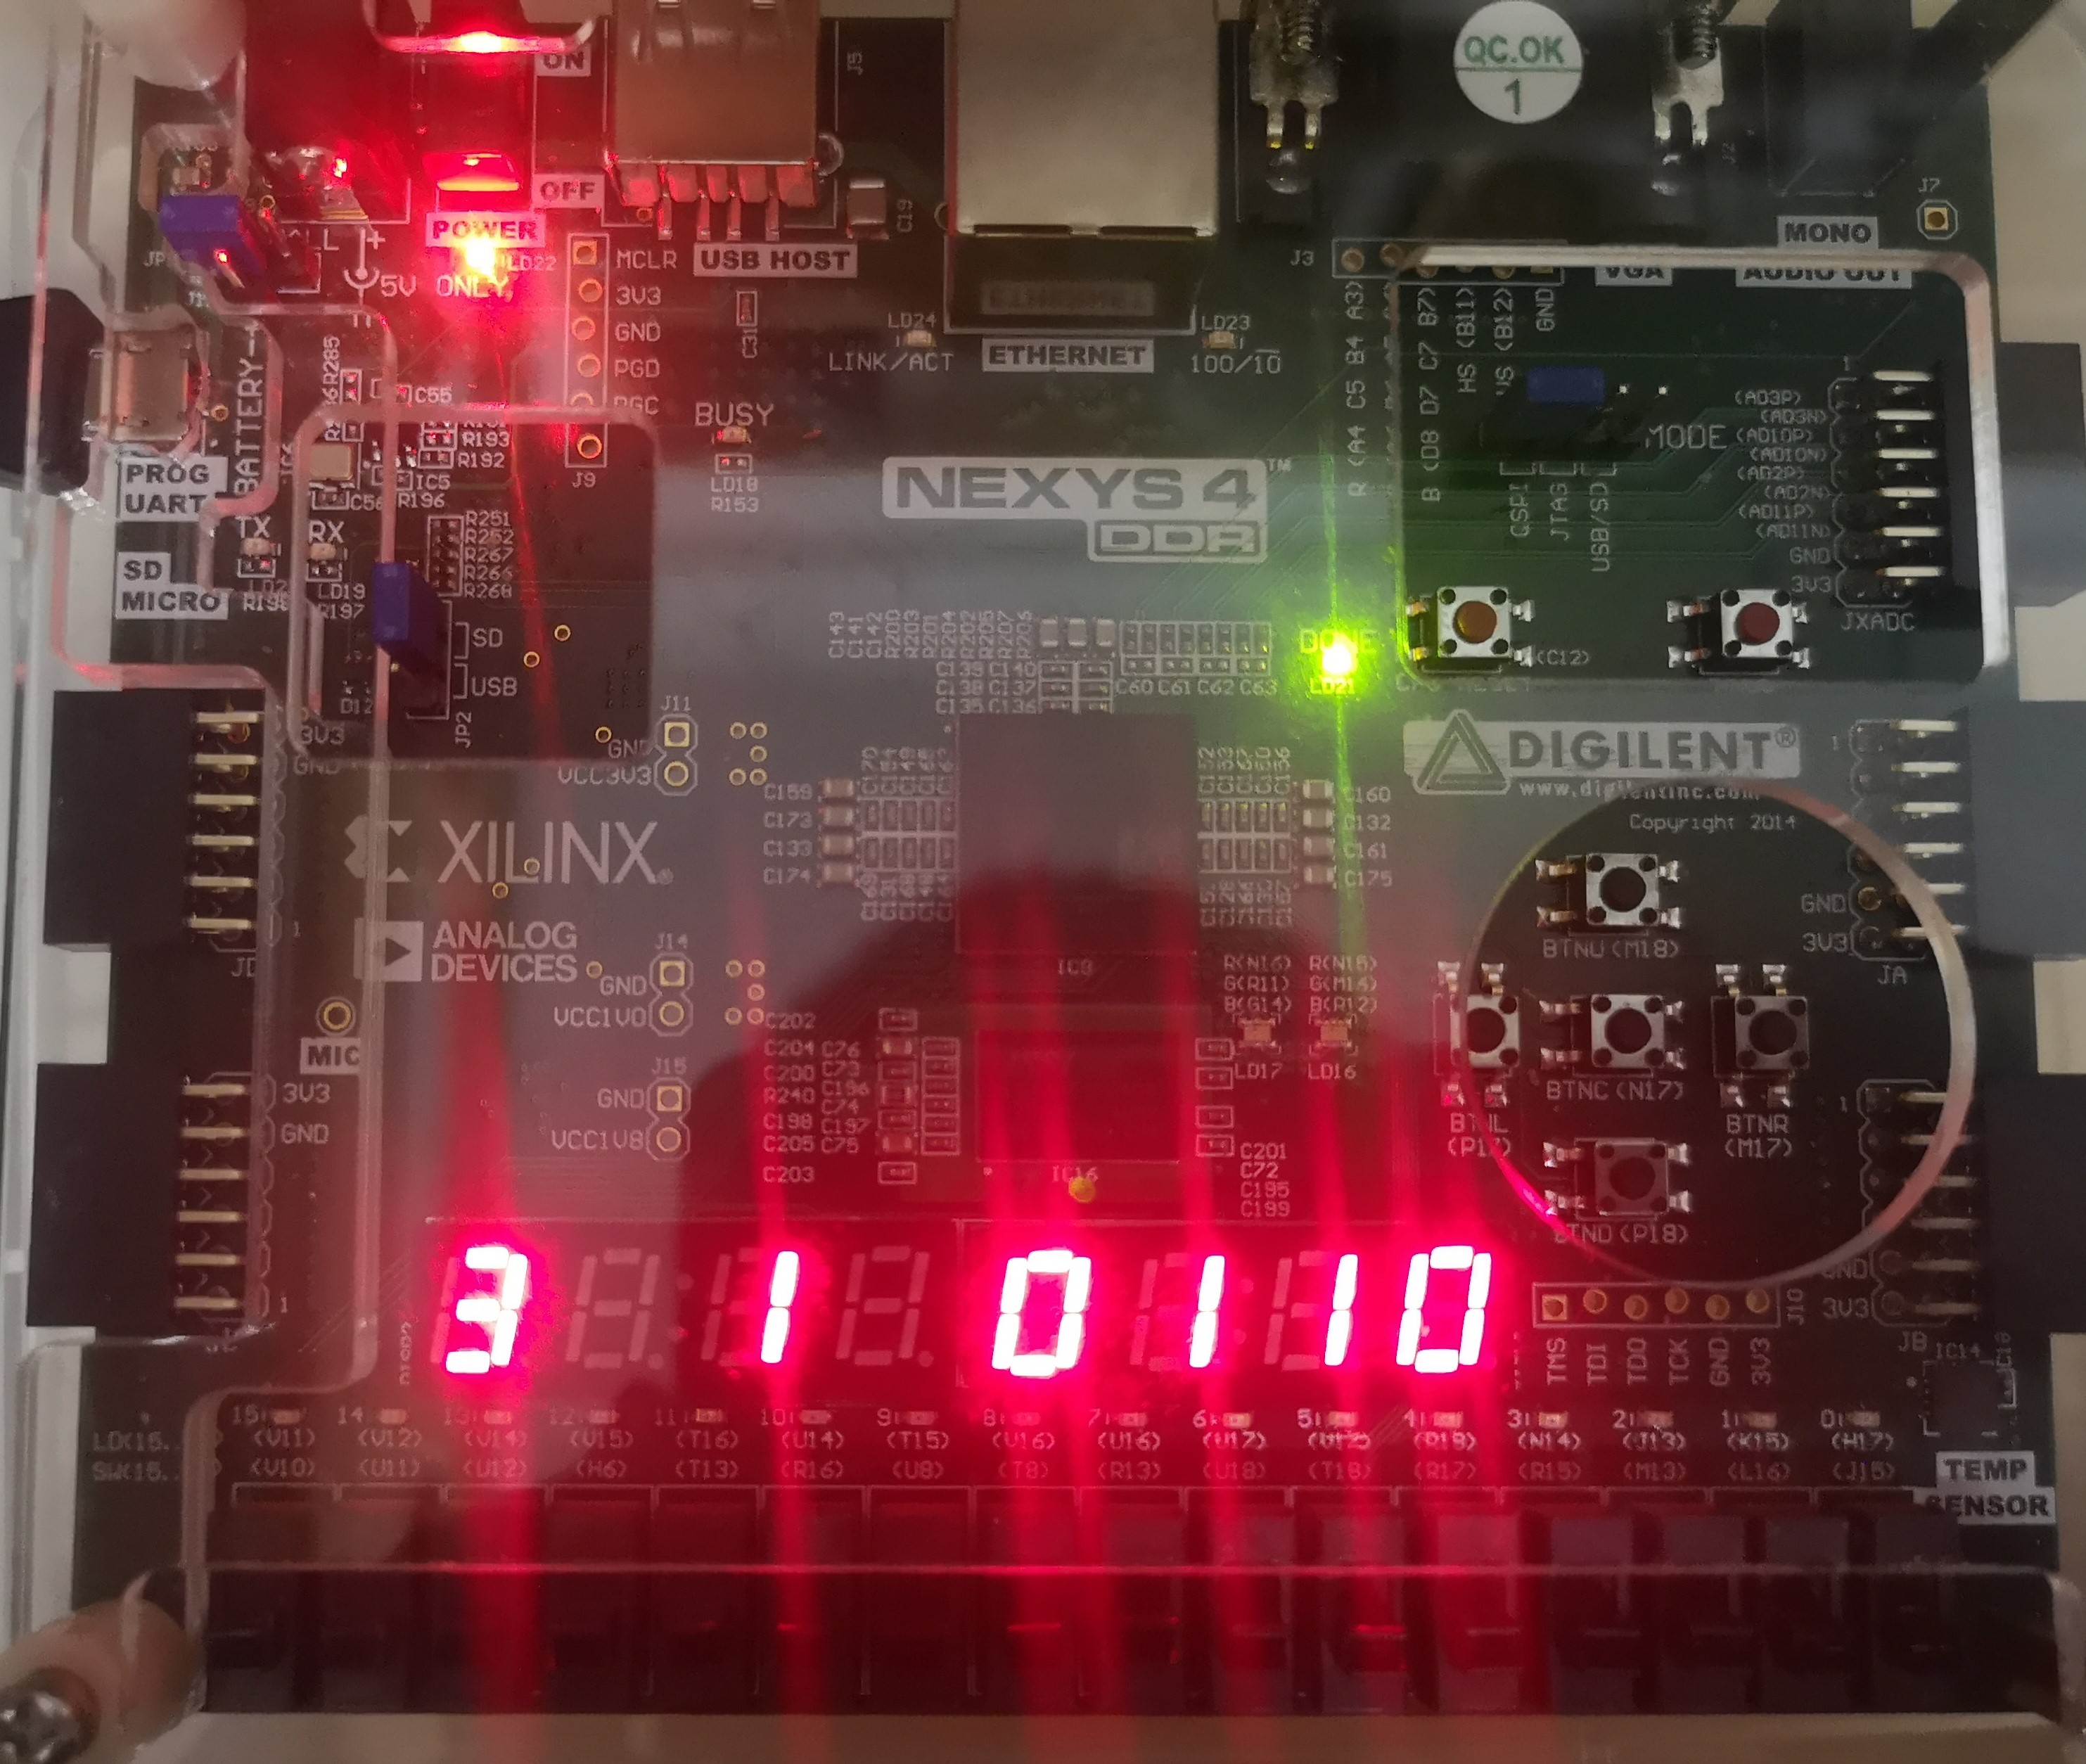
\includegraphics[scale=0.08]{e4_1.jpg}
			\label{e4_1}
		\end{minipage}
		\qquad
		\begin{minipage}[H]{0.48\linewidth}
			\centering
			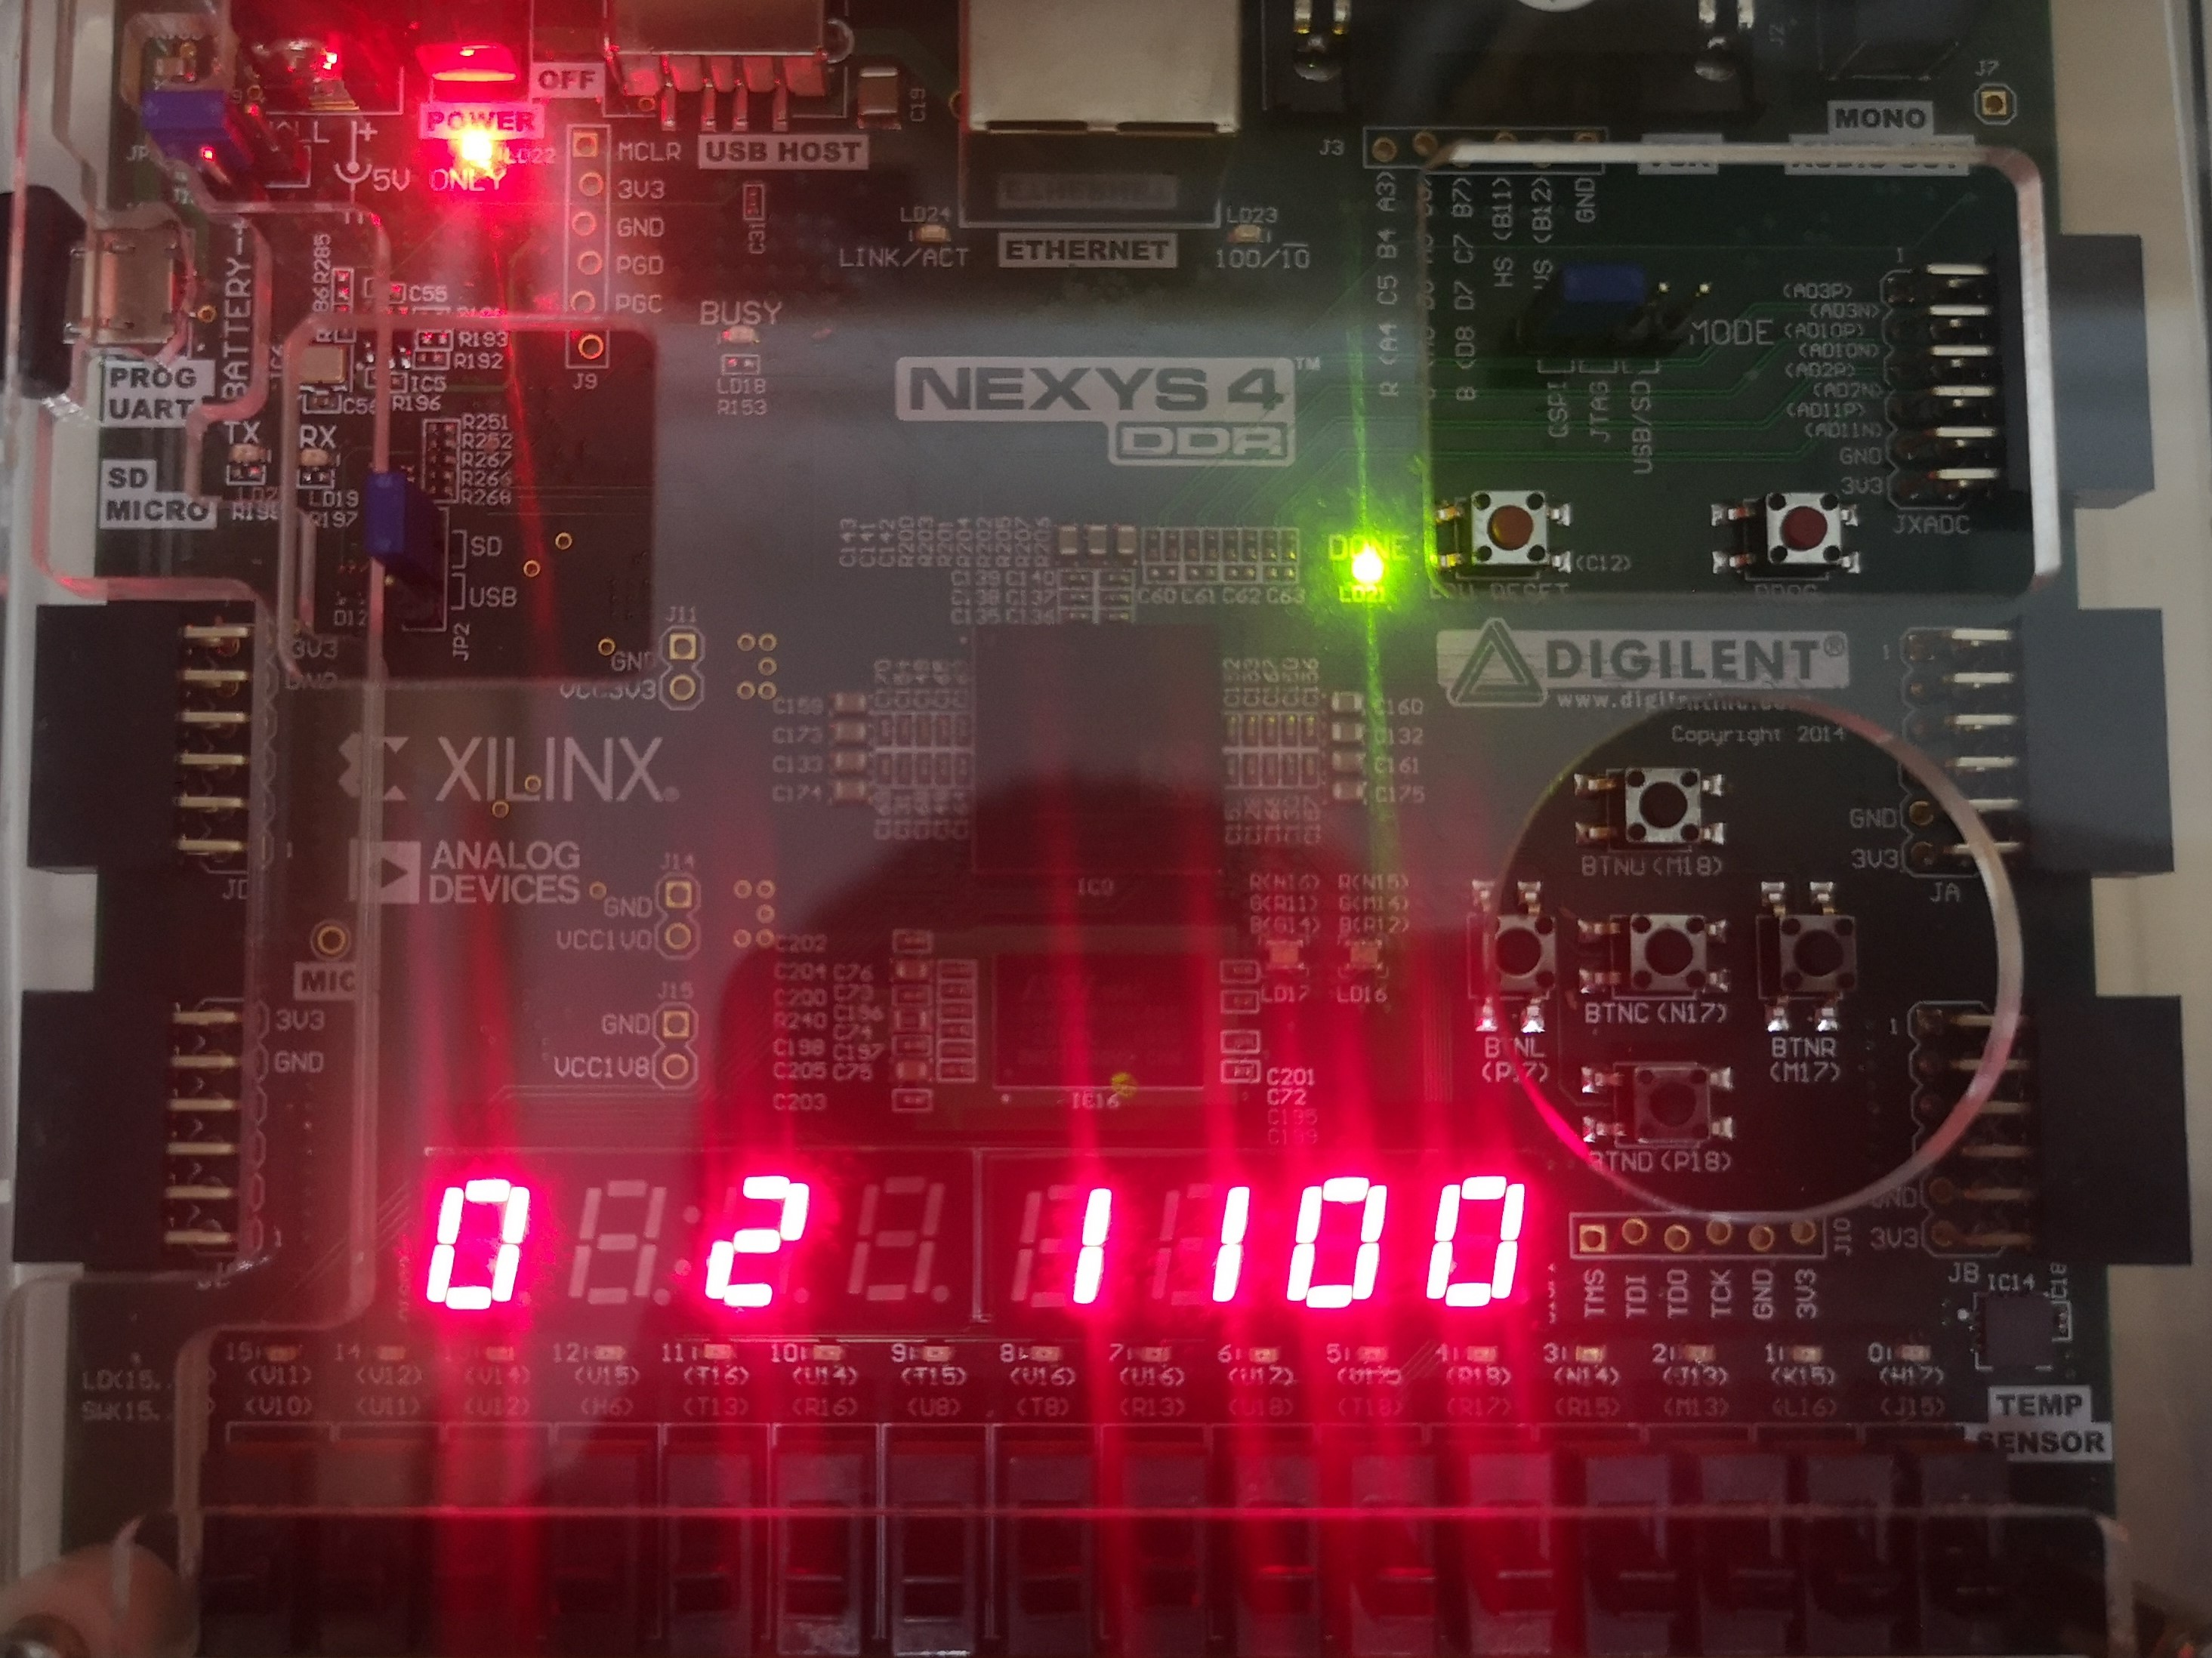
\includegraphics[scale=0.08]{e4_2.jpg}
			\label{e4_2}
		\end{minipage}
	\end{figure}
	状态图如下图:\par
	其中边上的值为:\textbf{输入/输出}。输出为1表示检测到序列。
	\begin{figure}[H]
		\centering
		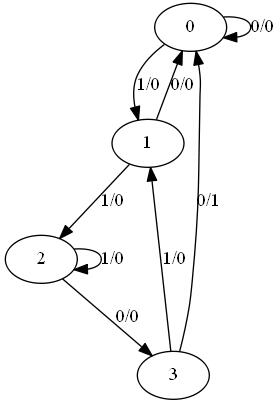
\includegraphics[width=0.5\linewidth]{e4_state_graph.jpg}
		\label{e4_state_graph}
	\end{figure}\par

	
	
	\section{总结与思考}	
	\subsection{本次实验的收获}
	在本次实验中,收获较大,学会了一些信号的处理分析,并且了解了有限状态机的搭建流程。\par
	
	\subsection{评价本次实验的难易程度}
	本次实验内容难度适中。\par
	
	\subsection{评价本次实验的任务量}
	本次实验任务量较大。\par
	
	\subsection{为本次实验提供改进建议}
	整个课程耗时较多,建议增加学分。\par
	
	
\end{document}
